\section{分析結果}
実験後,分析を行った結果,下の図に示すように,テスト2,3ではフィードバック利用回数が減少したとともに,テスト1,3の統制群にあった外れ値が実験群では無くなった.
ポストテストの結果では,テスト1では有意な結果が得られなかったが,テスト2,3では統制群に比べ実験群の方が点数が高くなった.さらに,T検定を行ったの結果,テスト3ではp<0.1となったため,有意傾向にあることが分かった.
認知負荷アンケートでは,統制群より実験群の方が色情報によるヒントが減少しているため,実験群の方が内在性負荷・外在性負荷において高くなったため,複雑であるという結果が得られた.学習関連負荷の項目では,テスト1はほとんど変化がなかったが,テスト2,3では実験群の方が高くなったため,学習に役立ったことが分かった.
フロー理論アンケートでは,学習の増加において有意である結果が得られたため,学習者は学習したという実感が得られていることが分かった.
テスト2,3のフィードバック利用回数の減少,ポストテスト3がp<0.1となり有意傾向にある,アンケートの結果から学習した実感が得られているというこの3点から難易度の高い問題において本研究の2色のフィードバックは有用であるといえる.

\begin{figure}[tb]
	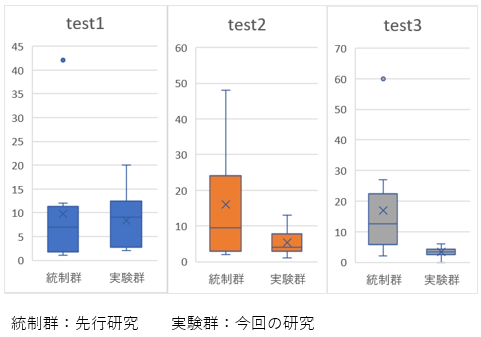
\includegraphics[width=0.9\linewidth]{tex1.png}
	\centering
	\caption{フィードバック利用回数}
	\label{fig1}
\end{figure}

\begin{figure}[tb]
	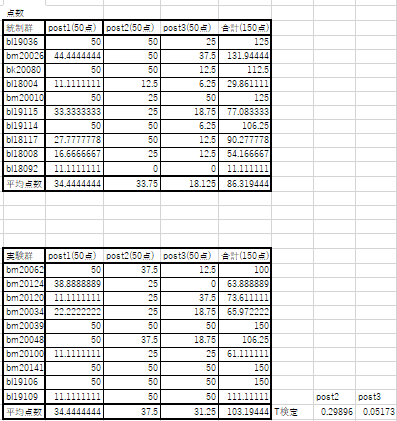
\includegraphics[width=0.9\linewidth]{tex2.png}
	\centering
	\caption{ポストテスト点数・T検定}
	\label{fig1}
\end{figure}